\documentclass[a4paper,twoside,12pt]{book}

\usepackage[french]{babel}

\usepackage{fontspec}
\setmainfont{Junicode} % Choisissez une fonte sérif lisible (Latin Modern, Junicode, Times)

\usepackage{hyperref}

%Module d'usage facultatif permettant d'intégrer les tables, index, bibliographie, automatiquement à la table des matières
\usepackage{tocbibind}
%\usepackage{lscape}

\usepackage{graphicx}

\usepackage[margin=2.5cm]{geometry}
\usepackage{setspace}
\setlength{\parindent}{1cm}
\onehalfspacing

%%%Pour les tableaux
%\usepackage{multirow}


%%% Les index
%\usepackage{makeidx}
%\usepackage{multind} %Ou splitidx
%\usepackage{index} %…
%\makeindex
%\makeindex{edition}
%\makeindex{texte}
%\newindex{etude}{adx}{and}{Index de l'étude}
%\newindex{edition}{bdx}{bnd}{Index de l'édition}



%%%Édition critique
%\usepackage{eledmac}
%\usepackage{eledpar}

%\footparagraph{A}

%\renewcommand{\Rlineflag}{D}

\hyphenation{}


\usepackage[babel]{csquotes}

\usepackage[backend=biber, sorting=nyt, style=enc]{biblatex}
\addbibresource{biblio/references.bib}



\usepackage{enumerate,lettrine}

\title{Normes typographiques pour les mémoires}
\author{Jean-Baptiste Camps}


\begin{document}


%\begin{abstract}

\frontmatter

\begin{titlepage}
\begin{center}

\bigskip

\begin{large}
UNIVERSITÉ PARIS, SCIENCES \& LETTRES
\end{large}
%TODO: nom établissement de préparation
\begin{center}\rule{2cm}{0.02cm}\end{center}

\bigskip
\bigskip
\bigskip
\begin{Large}
\textbf{Prénom Nom}\\
\end{Large}
\begin{normalsize} \textit{licencié ès lettres}\\
 (et les autres titres éventuels:)\\
\textit{Maître ès lettres}\\
\textit{Diplômé de master}\\
etc.
\end{normalsize}

\bigskip
\bigskip
\bigskip

\begin{Huge}
\textbf{TITRE DU MÉMOIRE}\\
\end{Huge}
\bigskip
\bigskip
\begin{LARGE}
\textbf{SOUS-TITRE}\\
\end{LARGE}

\bigskip
\bigskip
\bigskip
\begin{large}
\end{large}
\vfill

\begin{large}
Mémoire 
pour le diplôme de master [\textit{pour les M2}]\\
de première année de master\\
\og Humanités numériques et computationnelles \fg{} \\
\bigskip
2018
\end{large}

\end{center}
\end{titlepage}

\thispagestyle{empty}

\cleardoublepage

\section*{Résumé}
\addcontentsline{toc}{chapter}{Résumé}

 Résumé d'une trentaine de lignes à placer en tête du mémoire, accompagné d'une dizaine de mots-clés destinés à décrire le mémoire et des informations bibliographiques nécessaires pour le citer. Ce résumé et ces mots-clés sont destinés à compléter la notice bibliographique du mémoire dans la future bibliothèque numérique des mémoires.\\
N.B.: ne pas dépasser, au grand maximum, une page pour le tout.

\medskip

\textbf{Mots-clés:} Liste d'une dizaine de mots-clés, séparés par des points-virgules.

\textbf{Informations bibliographiques:} Prénom Nom, \textit{Titre du mémoire: sous-titre}, mémoire de master [1 ou 2] \og Humanités numériques et computationnelles\fg{}, dir. John Smith et Marie Schmitt, Université Paris, Sciences \& Lettres, 2018.

%TODO: demander résumé et mots-clés en anglais.

\section*{Abstract}
\addcontentsline{toc}{chapter}{Abstract}

Same abstract, but in English this time.

\medskip

\textbf{Keywords:} Liste d'une dizaine de mots-clés, séparés par des points-virgules.

\textbf{Bibliographic Information:} Forename Last-Name, \textit{Title: Subtitle}, M.A. thesis \og Digital and computational humanities\fg{}, dir. John Smith  and Marie Schmitt, Université Paris, Sciences \& Lettres, 2018.


\clearpage
\thispagestyle{empty}
\cleardoublepage


\section*{Remerciements}
\addcontentsline{toc}{chapter}{Remerciements}

\lettrine{M}{es remerciements} vont tout d'abord…

\clearpage
\thispagestyle{empty}
\cleardoublepage

\chapter*{Introduction}
\addcontentsline{toc}{chapter}{Introduction}

Ce document présente et synthétise des normes et conseils pour la préparation des mémoires (et mini-mémoires) du master Humanités numériques (PSL).

\printbibliography

\mainmatter

\part{Titre de la première partie du corps du document}

\chapter{Normes et conseils pour les mémoires}
%\markboth{\textsc{Normes et conseils pour les mémoires}}{}
%Titres courants

Pour tout ce qui est de l'ordre des règles typographiques, des normes bibliographiques et de la structure d'ensemble des mémoires, vous pouvez vous reporter aux livrets de conseil 3 à 5 des thèses d'archiviste paléographe\footcites{smith_conseils_3,smith_conseils_4,smith_conseils_5}.
Si la typographie vous intéresse, vous pouvez aussi consulter  l'excellent petit  précis :
\textsc{Imprimerie nationale}, \textit{Lexique des règles typographiques en usage à l'Imprimerie nationale}, Paris, 2002. 
Ce qui suit ne se substitue nullement à ces documents, mais en reprend des points essentiels et en précise d'autres propres aux mémoires de master.


\section{Mise en page}
\textbf{Recto-verso}. -- Composition \textbf{justifiée}. -- Pagination simple (arabe) ou double (romaine, puis arabe) si nécessaire. -- Marges du haut, du bas, intérieure et extérieure: 2,5\,cm. -- Caractère Times 12 ou équivalent. -- Interligne 1,5.\,-- Alinéa de 1\,cm pour les paragraphes (sans espacement entre les paragraphes); titres courants par chapitre au moins; citations longues (plus de 4 lignes) \textbf{détachées du corps du texte et indentées} (sans guillemets pour celles-ci, par opposition à celle présentées en ligne).

%\clearpage


\section{Structure du mémoire}

\begin{itemize}
	\item Page de titre et parties liminaires, dont: 
	\begin{itemize}
		\item résumé et mots-clés; 
		\item éventuelle épigraphe; 
		\item remerciements; 
		\item introduction; 
		\item bibliographie.
	\end{itemize}
	 \item Corps du document, subdivisé en parties et chapitres, et suivi d'une conclusion.
	 \item Annexes (dont documentation technique, documents divers, code commenté, planches, etc.). \item Parties finales, dont: 
	éventuels index, glossaire,\dots{}  table des figures et illustrations, table des matières.
\end{itemize}

et surtout: \textbf{annexes numériques} (données, scripts, documentation, modèles, etc.) structurées en \textbf{dossiers et sous-dossiers} et avec un fichier \texttt{README.md}.




\section{Bibliographie}


\subsection{Contenu et structuration}

La bibliographie est une partie \textbf{importante} de votre travail. Elle reflète votre appropriation de l'état de l'art et votre connaissance du domaine. Votre jury la lit. Ne la bâclez pas.

Un minimum de structure peut être utile, notamment si vous ne vous appuyez pas uniquement sur des travaux de recherche. Elle peut inclure des sections consacrées aux: sources; logiciels, modèles et spécifications techniques; travaux de recherche. Cette dernière peut être subdivisée, si cela s'y prête, selon des critères thématiques ou une typologie appropriée (par ex., «\,méthodologie\,» ou «\,méthodes computationnelles\,», \og{}Féodalité\fg{}, \og{}Histoire de l'art tibétain\fg{}, etc.).

Elle ne peut se limiter à quelques références, ni aux seules publications francophones, et ne peut en aucun cas se passer totalement tant de travaux historiques traditionnels que de travaux en \og{}humanités numériques\fg{} publiés dans les principales revues (\textit{DSH}, \textit{DHQ}, …) ou conférences du champ.

En revanche, elle ne se subdivisera en aucun cas selon le type de publication (monographie, article, actes de colloque) ou le seul support (numérique, imprimé,…).

\subsection{Mise en forme}

L'utilisation des normes de l'École des chartes est encouragée. 
Pour les utilisateurs du module \textit{Zotero} pour LibreOffice ou Word, un fichier de style \textsc{csl} est disponible sur l'Intranet. Pour les utilisateurs de \textsc{Bib}\LaTeX{}, un style (\textsc{bbx} et \textsc{cbx}) est également à votre disposition: il fait désormais partie des distributions \LaTeX{}, sous le nom \texttt{biblatex-enc} (\url{https://ctan.org/pkg/biblatex-enc}) et ses sources sont disponibles sur \texttt{Github} (\url{https://github.com/Jean-Baptiste-Camps/biblatex-enc}).

\section{Annexes numériques}

Les annexes numériques ont une très grande importance, presque autant que le mémoire qu'elles accompagnent. 

\textbf{Leur absence peut entraîner le refus du mémoire}.

Elles comprendront au moins,
\begin{itemize}
	\item le corpus et les jeux de données numériques utilisés pour la recherche;
	\item les scripts de manipulation des données et les protocoles d'analyse, les modèles;
	\item la documentation nécessaire;
	\item les autres documents que vous jugerez bon d'y inclure.
\end{itemize}


L'ajout de ces pièces doit permettre au lecteur de \textit{reproduire} et vérifier les analyses que vous avez effectuées.

Ex. de pièces: fichiers \texttt{csv}, bases de données, les fichiers \textsc{xml} produits et leur schéma, le manuel d'encodage, les scripts R, Rmd ou Python, etc.

Les pièces seront structurées par dossier et sous-dossiers, avec, à leur racine, un fichier \texttt{README.md}.

La documentation technique devra  comprendre une présentation de l'ensemble des fichiers fournis, et des scripts utilisés, 
de l'installation à l'utilisation.
Le rôle de chacun des fichiers de script ou programme devra être spécifié, les fichiers de paramétrage devront être présentés.
Les fichiers de code devront être commentés pour faciliter leur compréhension.

N.B.: attention à la compatibilité des programmes et fichiers livrés avec les différents systèmes d'exploitation (et les différents navigateurs).

Les annexes numériques seront fournies via un lien à un entrepôt (\texttt{Github} par exemple, ou mieux encore, Zenodo et autres archives de données de recherche), si les droits le permettent, et sinon sur une clé (éviter CD-ROM ou cartes perforées).

\section{Dépôt du mémoire}

\subsection{Avant la soutenance}

En M2, le mémoire doit être rendu au plus tard trois semaines avant la date prévue de soutenance, en autant  d'exemplaires que de membres du jury (trois, sauf cas particuliers). En M1, ils doivent être rendus pour le 1\ier{} juin.

Pour le dépôt électronique, les formats de fichiers acceptés sont, pour les fichiers source, les formats OpenDocument (.odt) ou \LaTeX{} (.tex), obligatoirement accompagnés d'une compilation \textsc{pdf}, ainsi que de tous les livrables techniques et fichiers d'accompagnement nécessaires.

\subsection{Pendant la soutenance}

La soutenance en elle-même (M2 uniquement) dure environ une heure. Le ou la candidate y présente ses recherches (historique du sujet, démarche, éventuelle rapide égo-histoire, conclusions principales, limites, etc.) pendant une quinzaine de minutes (max. 20 minutes), puis les trois membres du jury (directeurs ou directrices thématique, numérique, et président du jury) prennent la parole à leur tour pour questions et remarques.

\begin{figure}
\centering %
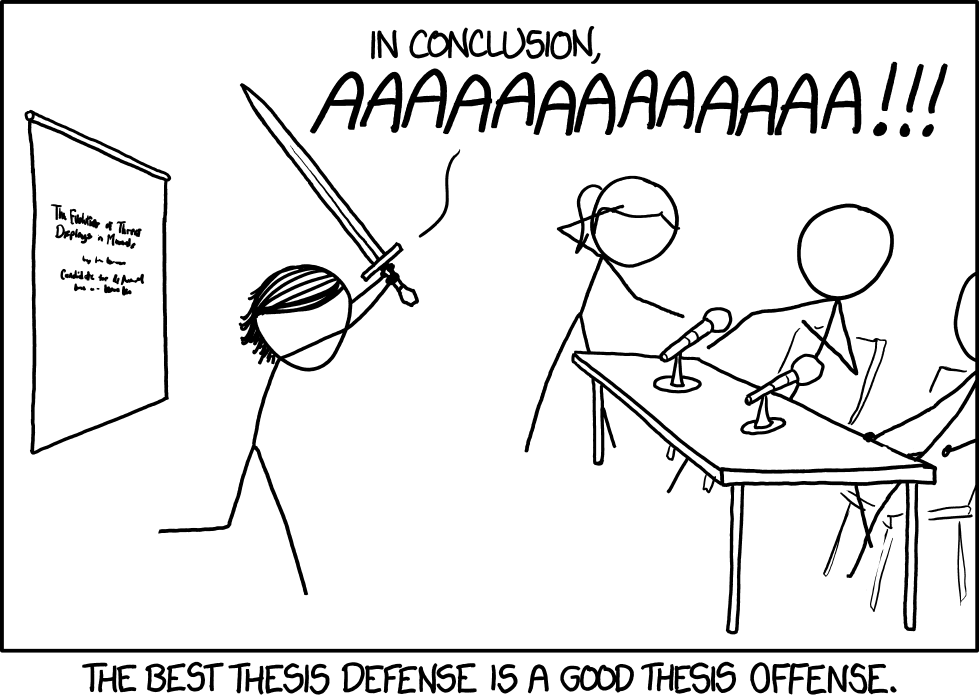
\includegraphics[width=0.75\textwidth]{img/thesis_defense_2x.png}
\caption{Randall Munroe, \textit{Thesis Defense}, XKCD 1403, \url{https://xkcd.com/1403/}.}
\end{figure}


\subsection{Après la soutenance}

Dans la perspective d'une publication en ligne du mémoire sur une archive ouverte, à l'issue de la soutenance, le jury précisera si le mémoire peut-être publié en l'état, s'il doit faire l'objet de corrections ou s'il ne peut être publié. Il appartient alors à l'auteur du mémoire 
de fournir la version corrigée, sous forme électronique (OpenDocument ou \LaTeX{} et \textsc{pdf}, accompagnés des livrables s'ils ont été modifiés) et de signer une autorisation de diffusion.

\section{Quelques conseils généraux}

Pour les M2, le mémoire est l'aboutissement de vos études de master --\,voire le premier pas vers une thèse de doctorat\,-- et il est également le travail dans lequel vous avez le plus d'autonomie et de liberté. 
Il importe néanmoins de faire un point régulier sur l'état d'avancement de vos travaux avec vos directeurs. Dans le cadre de l'emploi du temps assez resserré de la deuxième année du master, il est souhaitable
de commencer à concevoir, organiser et rédiger son mémoire le plus tôt possible.


Si les mémoires ne sont pas jugés sur la quantité de pages qu'ils contiennent, mais sur la qualité et rigueur de leur démarche scientifique et numérique, tant du point de vue des sujets abordés que de la méthode (données, outils d'analyse, etc.). Pour le M1, une trentaine de pages est suffisante; en M2, 80 pages peuvent suffire, si elles sont claires, bien construites et fondées sur une démarche pertinente.
Il s'agit là toutefois d'indications et non pas de règles absolues.

Le mémoire doit être rédigé dans une langue claire et rigoureuse, évitant les anglicismes ou le jargon. Il s'adresse à un public relativement large et a vocation à pouvoir être diffusé en ligne. À ce titre, d'une part, la qualité de son contenu vous engage autant que PSL et, d'autre part,  
le texte du mémoire doit être clair et compréhensible, tant que faire se peut, par des chercheurs même non spécialistes du sujet traité. 
Les concepts, normes, outils,\dots{} mentionnés devront être définis et présentés.
Tous les tableaux et illustrations devront être légendés (et repris dans la table des illustrations).

\paragraph{Note finale:} La majeure partie de ces règles a pour but de favoriser la lisibilité et la clarté du texte, qu'il importe également de ne pas surcharger d'artifices typographiques (gras, tirets, emploi abusif des majuscules, etc.) qui en rompraient la lisibilité, pas plus que d'abréviations (en dehors des plus courantes) ou de jargon.

\paragraph{Sources et citations:} On rappellera qu'il est absolument impératif, d'un point de vue éthique, scientifique et légal, de \textit{citer} toutes les ressources utilisées, d'identifier correctement les citations et de les \textit{attribuer} à leurs auteurs (cela vaut aussi pour les figures et graphiques, qui doivent être légendés). Le plagiat est une fraude susceptible de sanctions (la moindre étant la non obtention du diplôme).



\appendix
\part*{Annexes}
\chapter{Titre du premier chapitre d'annexes}
\section{Notes de l'atelier sur les mémoires de M1}

\subsection{Le mémoire}\label{le-muxe9moire}

\subsubsection{Qu'est-ce qu'un mémoire?}\label{quest-ce-quun-muxe9moire}

Un mémoire = une question (dont on a pas encore la réponse ou dont la
réponse n'est pas satisfaisante). Les données et le protocole d'analyse découlent de la question, pas l'inverse (i.e., 'je vais faire du réseau, mais sur quoi?'). Ne pas prendre la démarche à l'envers.

\textbf{Identifier une question sur laquelle une démarche de HN peut être pertinente: pas une micro analyse quali, mais quelque chose sur laquelle une approche sérielle, macro, ou avec une granularité très fine, etc., peuvent être pertinente. Ou il y a un besoin d'objectivation. 
	Tout ne s'y prête pas.}

Attention: \emph{il est bien souvent impossible d'identifier une question de ce type sans une connaissance très fine d'un domaine d'études et une certaine expérience de la recherche} que l'on n'a pas forcément encore acquise au moment de définir son sujet de mémoire. C'est pour ça qu'il est important que le sujet soit conçu par ou co-conçu avec des directeurs et directrices de recherche spécialisés en méthodes numériques et sciences humaines.

\textbf{Introduction}

\begin{itemize}
	\item
	introd. question, l'expliquer;
	\item
	pourquoi est-elle pertinente?
\end{itemize}

\textbf{État de l'art}

\begin{itemize}
	\item
	Que sait-on sur le sujet?
	\item
	Quelles tentatives de réponse jusque là? Quelles limites?
	\item
	bibliographie du sujet: comment faire un bibliogr. en HN (et en général)? Quelles sources de données (aperçu général des publications du champ: revues, actes, manuels, … articles de recherche / de synthèse)? Quels moteurs de recherche bibliographique (Google Scholar)? Lire en anglais (notamment). Quels outils de gestion de bibliographie (BDD, styles, etc.)? 
	\item dépouillements systématiques + bibliographie par rebond (citations, etc.);
\end{itemize}

\textbf{Démarche}

\begin{enumerate}
	\item
	(quoi) données:
\end{enumerate}

\begin{itemize}
	\item
	pourquoi celles-ci? quelle est leur utilité pour répondre à la
	question? Quelles limites/biais?
	\item 
	collecte des données;
	\item
	formalisation et sa pertinence;
\end{itemize}

\begin{enumerate}
	\def\labelenumi{\arabic{enumi}.}
	\setcounter{enumi}{1}
	\item
	(comment) méthode:
\end{enumerate}

\begin{itemize}
	\item
	quelles méthodes possibles? Pourquoi celle-là (avantages/utilité)? Que
	peut-on en attendre (limites, biais)?
	\item
	En quoi consiste-t-elle?
\end{itemize}

\begin{enumerate}
	\def\labelenumi{\arabic{enumi}.}
	\setcounter{enumi}{2}
	\item
	résultats
\end{enumerate}

\begin{itemize}
	\item
	Quels éléments de réponse a-t-on obtenu?
	\item
	Qu'en déduire?
	\item
	Que reste-t-il à faire
\end{itemize}

\textbf{Conclure}

Résultats majeurs, leurs limites, etc.

\subsubsection{Attendus}\label{attendus}

\begin{itemize}
	\item
	Un texte d'une trentaine de pages (avec graphiques, tableaux, etc.);
	\item
	des annexes numériques:
	\item
	données;
	\item
	scripts, requêtes, etc.
\end{itemize}

\subsubsection{Forme}\label{forme}

cf.~document de forme

\subsection{Un état de l'art en humanités numériques}


\begin{itemize}
	\item Quelles sont les principales revues du champ?
	\item les principales conférences (et les sociétés savantes qui les organisent)?
	\item où trouver de l'information bibliographique?
\end{itemize}

\paragraph{Pour le prochain atelier:}
préparer une petite bibliographie commentée de 5 références méthodologiques (en HN) et 5 thématiques (``traditionnelles'' ou HN).


\backmatter

\listoffigures
\tableofcontents

\end{document}
